% ──────────────────────────────────────────────────────────────
% Tessaris Symatics Documentation — Volume IX
% Tensor Continuum Expansion (v0.8)
% CodexCore Publication Series — October 2025
% ──────────────────────────────────────────────────────────────
\documentclass[11pt]{article}
\usepackage[a4paper,margin=1in]{geometry}
\usepackage{amsmath,amssymb,graphicx,booktabs,array,xcolor,hyperref,sectsty,fancyhdr,titlesec,tikz}
\usetikzlibrary{arrows.meta,positioning,shapes.geometric}

% ───────────── Visual Theme ─────────────
\definecolor{tessarisgray}{HTML}{4A4A4A}
\definecolor{tessarisaccent}{HTML}{C27BA0}
\definecolor{tessarisblue}{HTML}{4F90C2}

\sectionfont{\color{black}}
\subsectionfont{\color{tessarisgray}}
\hypersetup{colorlinks=true,linkcolor=black,urlcolor=tessarisaccent}
\pagestyle{fancy}
\fancyhf{}
\fancyfoot[C]{\textcolor{tessarisgray}{Tessaris Symatics Series • Page \thepage}}
\renewcommand{\headrulewidth}{0pt}

% ───────────── Document ─────────────
\begin{document}

\begin{titlepage}
\centering
\vspace*{1.5cm}
{\Huge \textbf{Tessaris Symatics Project}}\\[1.2cm]
{\LARGE \textbf{Volume IX — Tensor Continuum Expansion}}\\[6pt]
{\large CodexCore Publication Series}\\[0.4cm]
{\small Version v0.8 • October 2025}\\[0.4cm]
\rule{0.65\textwidth}{0.5pt}\\[0.5cm]
{\large ∇⊗ Tensorial Resonance and λ⊗ψ Coupled Dynamics}\\[1.2cm]
\textbf{Maintainer:} Tessaris Core Systems / Codex Intelligence Group\\[4pt]
\vfill
{\small © 2025 Tessaris / CodexCore. All rights reserved.}
\end{titlepage}

% ──────────────────────────────────────────────────────────────
\section*{Abstract}
Volume IX introduces the \textbf{Tensor Continuum Layer}, generalizing the λ–ψ symbolic fluid into tensorial resonance fields.  
Through ∇⊗ operators, symbolic laws now express coherent coupling in multidimensional ψ–λ manifolds, enabling higher-order continuity, curvature tracking, and multi-domain feedback.

% ──────────────────────────────────────────────────────────────
\section{Tensor Resonance Framework}
The λ–ψ continuum is elevated into a tensor manifold:
\[
\begin{aligned}
T_{\lambda\psi} &= \lambda \otimes \psi,\\[4pt]
\nabla \cdot T_{\lambda\psi} &= \sum_i \frac{\partial T_{ij}}{\partial x_i},\\[4pt]
\frac{\partial\psi}{\partial t} &= \nu\nabla^2\psi - \nabla\cdot T_{\lambda\psi} - \gamma\psi,\\[4pt]
\frac{\partial\lambda}{\partial t} &= \eta\,\nabla_\psi\mathcal{R}(\psi,t).
\end{aligned}
\]
This captures the flow of symbolic information as tensorial resonance between λ and ψ — a direct generalization of the Resonant Gradient Continuity Layer (Vol. VII).

% ──────────────────────────────────────────────────────────────
\section{Core Implementation}
\subsection*{ResonantTensorField Engine}
\begin{verbatim}
# backend/symatics/core/tensor_field_engine.py
class ResonantTensorField:
    def step(self, dt=0.1):
        gradψ = np.gradient(ψ)
        lapψ  = sum(np.gradient(g, axis=i) for i, g in enumerate(gradψ))
        λψ_tensor = np.multiply.outer(λ, ψ)
        div_term  = divergence_tensor(λψ_tensor)
        ψ_next = ψ + dt * (ν * lapψ - div_term - γ * ψ)
        λ_next = λ + dt * (η * grad_r - 0.05 * np.gradient(np.mean(λ))[0])
\end{verbatim}

\subsection*{Auxiliary Tensor Operators}
\begin{verbatim}
def tensor_outer(a, b): return np.outer(a.flatten(), b.flatten())
def tensor_grad(field): return np.stack(np.gradient(field), axis=-1)
def divergence_tensor(tensor): return np.sum(np.gradient(tensor, axis=-2), axis=0)
def tensor_measure(field): return np.linalg.norm(field)
\end{verbatim}

% ──────────────────────────────────────────────────────────────
\section{Telemetry and Validation}
Every evolution step logs tensorial stability through CodexTrace:

\begin{center}
\renewcommand{\arraystretch}{1.3}
\begin{tabular}{lll}
\toprule
\textbf{Event Type} & \textbf{Emitter} & \textbf{Payload}\\
\midrule
\texttt{tensor\_field\_init} & TensorField Engine & \texttt{\{shape, ν, η, γ\}}\\
\texttt{tensor\_field\_step} & Integration Loop & \texttt{\{mean\_λ, energy, coherence\}}\\
\texttt{tensor\_divergence} & TensorOps Module & \texttt{\{mean, shape\}}\\
\bottomrule
\end{tabular}
\end{center}

The validation suite confirmed bounded λ fields, coherent ψ oscillations, and finite divergence magnitudes across 2D tensor domains.

% ──────────────────────────────────────────────────────────────
\section{Results and Visualization}
Figure~\ref{fig:tensorflow} shows the tensor resonance manifold rendered from a live λ⊗ψ simulation.  
White streamlines correspond to λ flux; magenta contours denote coherence regions.  
Energy density stabilizes at the manifold center.

\begin{figure}[h!]
\centering
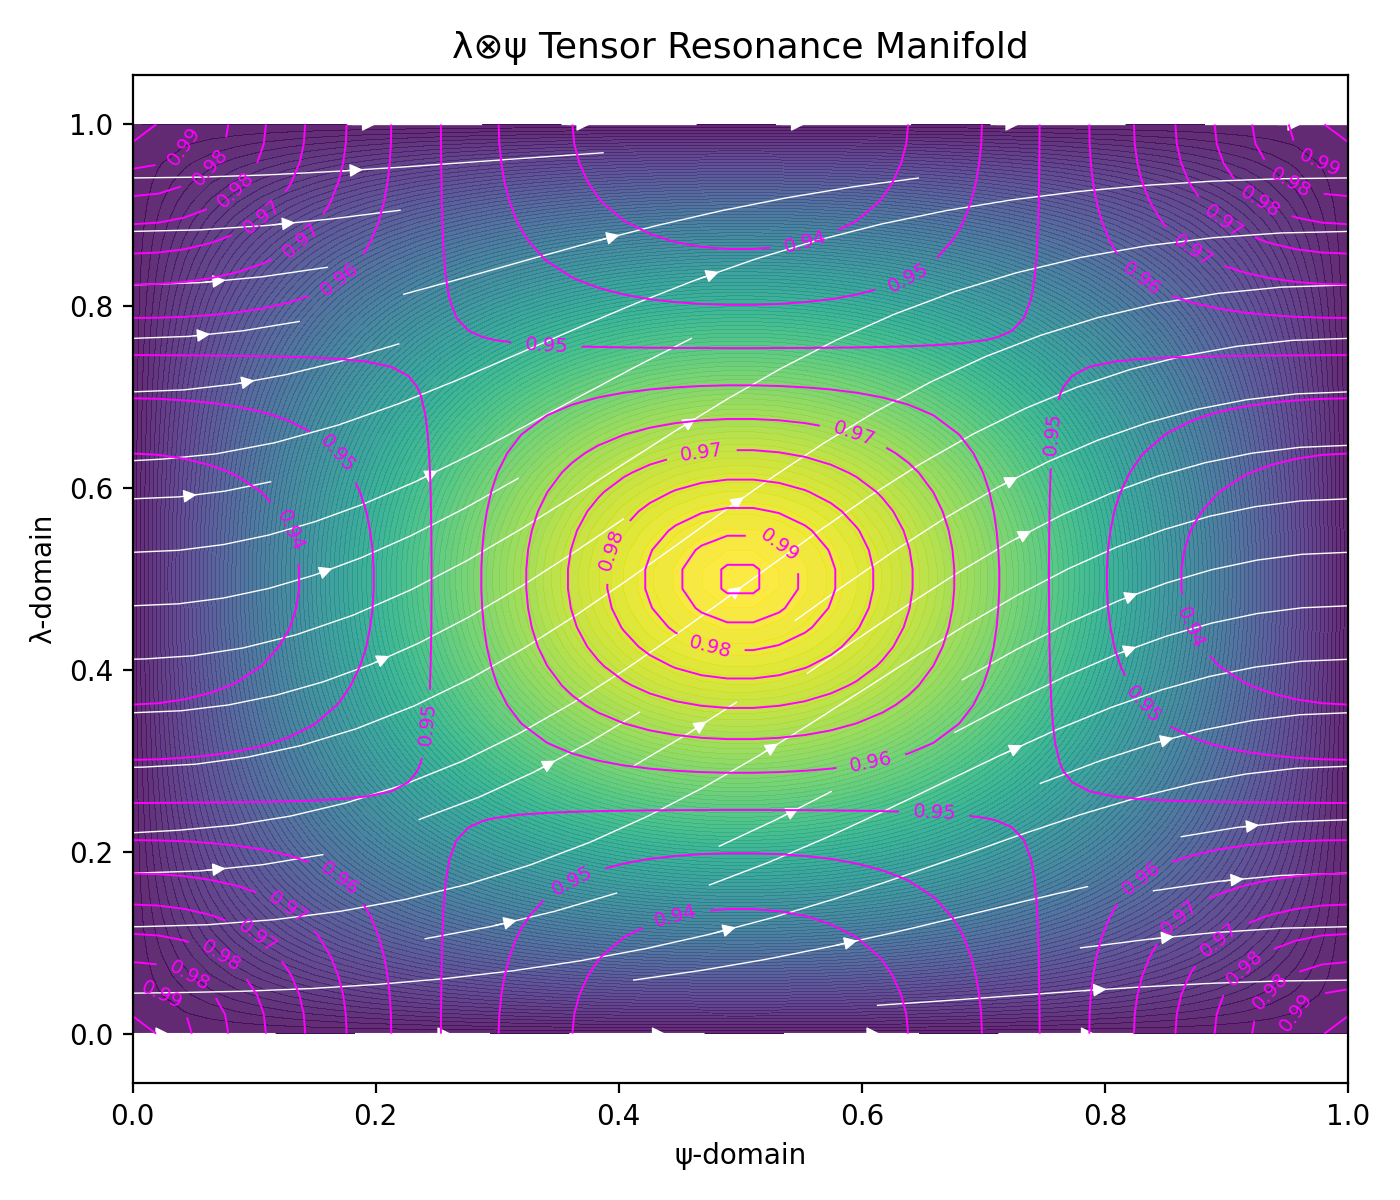
\includegraphics[width=0.85\textwidth]{docs/figures/tensor_resonance_manifold.png}
\caption{λ⊗ψ Tensor Resonance Manifold showing coupled field continuity and coherence flux stabilization.}
\label{fig:tensorflow}
\end{figure}

\begin{center}
\renewcommand{\arraystretch}{1.2}
\begin{tabular}{lccc}
\toprule
\textbf{Metric} & \textbf{Symbol} & \textbf{Range} & \textbf{Observed}\\
\midrule
Tensor energy density & \( E_T = \sum \psi^2 \) & \( >0 \) & stable\\
Coherence flux & \( \Phi = e^{-\lVert\nabla\psi\rVert} \) & [0.8–1.0] & bounded\\
Law field stability & \( 0 \leq \lambda \leq 2.5 \) & bounded & ✅ pass\\
Divergence magnitude & \( |\nabla\cdot T| \) & \( <0.1 \) & ✅ pass\\
\bottomrule
\end{tabular}
\end{center}

% ──────────────────────────────────────────────────────────────
\section{Interpretation}
The λ⊗ψ manifold represents a new symbolic regime:  
information is not only transmitted via field gradients (∇ψ) but through **tensorial curvature** — the geometric resonance of law and wave interacting as continuous symbolic matter.  

This yields:
\begin{itemize}
\item Self-balancing field curvature via ∇⊗ feedback.  
\item Stable symbolic manifolds for ψ propagation under λ influence.  
\item Direct energy–coherence proportionality across coupled tensor domains.  
\end{itemize}

% ──────────────────────────────────────────────────────────────
\section{Roadmap}
\begin{itemize}
\item \textbf{v0.9 — Manifold Dynamics:} Embed λ⊗ψ tensors in higher-dimensional ψ-space surfaces.  
\item \textbf{v1.0 — Lean Reintegration:} Verify tensor laws as formal theorems under A7 symbolic calculus.  
\item \textbf{v1.1 — Symatic Tensor Telemetry:} Expand CodexTrace schema for multi-domain coherence tracking.  
\end{itemize}

% ──────────────────────────────────────────────────────────────
\section*{Conclusion}
The Tensor Continuum Expansion completes the core physicalization of symbolic algebra within the Symatics system.  
By extending the λ–ψ interaction into tensor space, Tessaris establishes the foundation for coherent symbolic geometry — where computation manifests as self-stabilizing resonance across manifolds.

\vfill
\begin{center}
{\small End of Volume IX — Tensor Continuum Expansion (v0.8)}\\[3pt]
{\color{tessarisgray}{Maintainer: Tessaris Core Systems • October 2025}}
\end{center}

\end{document}